\section{Frontend}

Frontend of an application is what consumers see at first and the way to interact with the middleware. The biggest challenge was designing interfaces for everyone and not only for developers. User experience is the key success of every applications. 

\subsection{Technologies}


\subsubsection{AngularJS}

AngularJS is now the leader for dynamic view in web-application. It is support by Google and private. AngularJS strength is its two-way data binding. Whatever your are modifying, View or Model the other is updated instantly. However, the model is the single-source-of-truth for the application state.  AngularJS provide a high-level module to interact with RESTFul server called \emph{\$resource} and every CRUD function are defined easily. 

\subsubsection{Jade}
What is Jade? \emph{Jade is a high performance template engine heavily influenced by Haml and implemented with JavaScript for node and browsers.} In iFlux, Jade is used to create Angular partials because HTML is verbose. 


\subsubsection{Stylus}

Write CSS directly is not anymore done by web developers. CSS preprocessor technologies like Saas LESS or Stylus replace it and allow you to use variables, nesting, inheritance, mixins, importing, etc. Stylus is different from the two others by omitting brackets, colons and semi-colons in your code. The result of the preprocessor is a standard CSS file. 

\subsubsection{Grunt and Bower}
Grunt is a JavaScript task runner and allow you to define repetitive task and automate it, like compile Stylus, run the web server, process Jade, etc. We define a watch task that process Stylus file after each modification and integrates it on the running website. With that, your website has always the latest modifications. 

Bower is a package manager for the web stack. You define in \emph{bower.json} witch version of your components you want and it installed your package. Here is the dependencies of the frontend. There are lots of Angular modules provided by Angular or by users on Github. 

\begin{lstlisting}
{
  "name": "code",
  "version": "0.0.1",
  "ignore": [e
    "**/.*",
    "node_modules",
    "components"
  ],
  "private": true,
  "dependencies": {
    "angular": "~1.4.1",
    "angular-bootstrap": "~0.13.0",
    "angular-bootstrap-switch": "~0.4.1",
    "angular-mocks": "1.4.1",
    "angular-route": "~1.4.1",
    "angular-resource": "~1.4.1",
    "angular-sanitize": "~1.4.1",
    "angular-schema-form": "~0.8.2",
    "angular-ui-ace": "~0.2.3",
    "angular-ui-select": "~0.12.0",
    "bootstrap": "3.3.x",
    "fontawesome": "~4.3.0",
    "jquery": "~2.1.1",
    "ngstorage": "~0.3.6",
    "jquery-ui": "~1.10.4"
  },
  "resolutions": {
    "angular": "1.4.1"
  }
}
\end{lstlisting}

\subsection{UX design}
The masterpiece of UX design is a responsive website with the bootstrap technologie. We did not develop the frontend for a mobile because of the complexity of interfaces. Mobile phone are not usefull when you have to write JS expression, navigate to find the help or fill long form. However, the website is responsive for the different resolution of the screen. 

The concept of CRUD function is applied to the interface which for every parts of the model, has a management interface and an editor/view interaface. In the management view, you can create, read, update or delete an entry. We did not inovate for the presentation. 

\subsubsection{Event Source}
On the Event Source Template editor we employed the project \emph{Angular Schema Form} http://schemaform.io/ which allow you to create a dynamic Angular form based on the JSON Schema. To instantiate an event source the user have to provide a certain amont of data and he will do that through the dynamic form. It is the keystone of the frontend to configure dynamically distant objects or services. 

The below figure\ref{fig:iflux-event-source} is the management interface for Event Source Template and Event Source. 
\begin{figure}
\centering
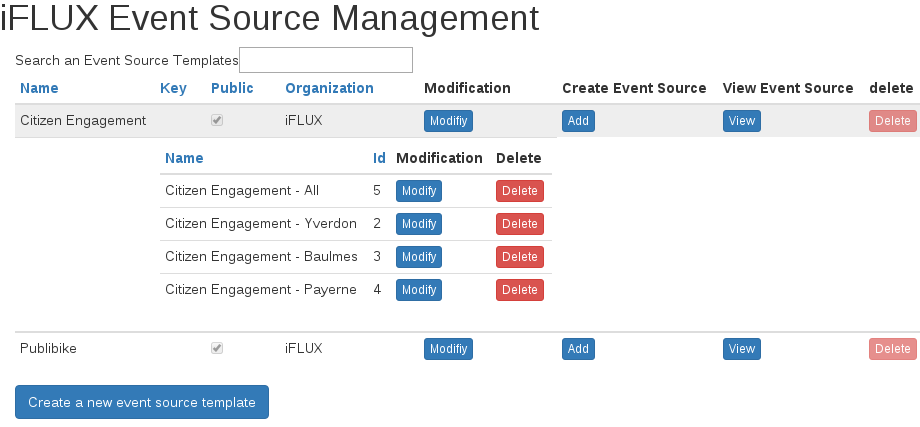
\includegraphics[width=1\columnwidth]{figures/eventSource.png}
\caption{Event Sources management}
\label{fig:iflux-event-source}
\end{figure}

\subsubsection{Action Target}

The Action Target interface is almost the same than Event Source. \emph{Angular Schema Form} is also used to define endpoints and configure them. 

\subsubsection{Rules}
To create a rules, you have to define a minium of one condition and one action. Of course, you can add as much as you want. Configure a rules is not an easy task. This is why modals views are bind to dropdown lists to help users to choose the right instance or the right action/event type. To write JS expression, a help box displays properties of the event based on the choosen event type. The figure\ref{fig:iflux-rules-action} below show an action box with the help - a part of the rules form. Javascript editor is based on \emph{Ace} which is an online code editor. It provide syntax highlighting, automatic indent, live syntax checker, etc. We make it resizable to allow a better visibility of your function.

\begin{figure*}
\centering
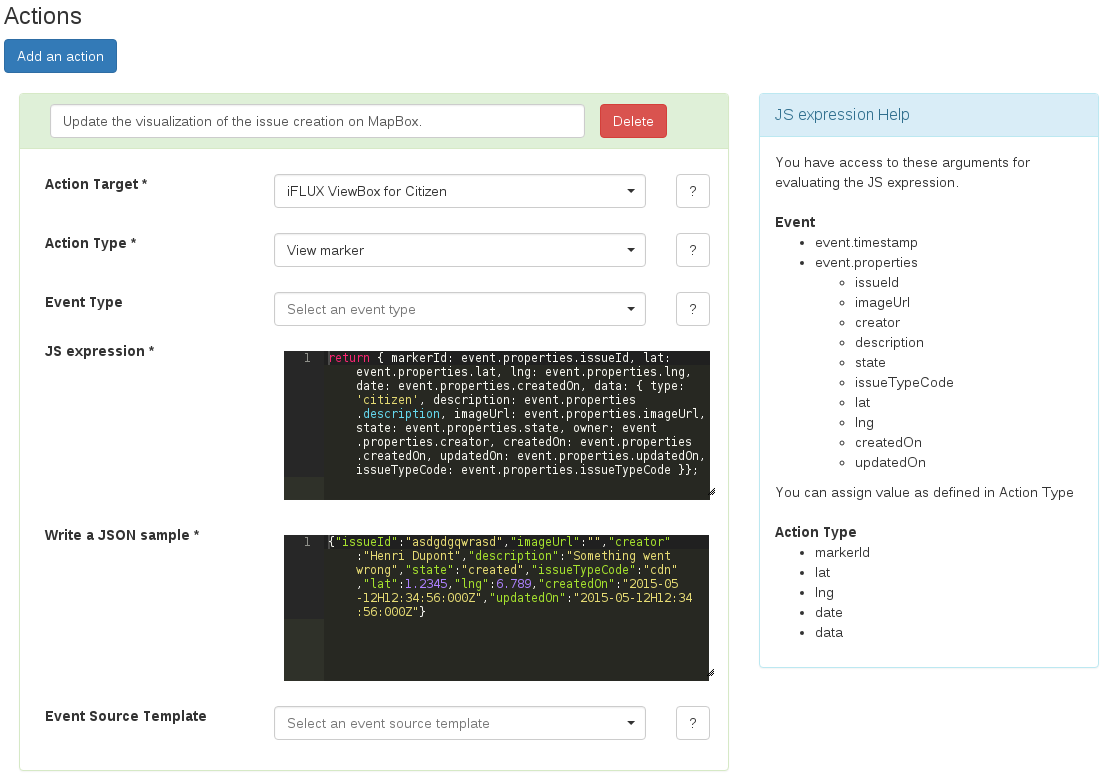
\includegraphics[width=0.9\textwidth]{figures/rules-transformation.png}
\caption{Rules editor - one action}
\label{fig:iflux-rules-action}
\end{figure*}
